\documentclass[12pt,a4paper]{beamer}
\usetheme{Montpellier}
\usepackage[utf8]{inputenc}
\usepackage[english]{babel}
\usepackage{amsmath}
\usepackage{amsfonts}
\usepackage{amssymb}
\usepackage{makeidx}
\usepackage{graphicx}
\usepackage{lmodern}
\usepackage{kpfonts}
\usepackage{fourier}
\usepackage{hyperref}
\usepackage{tipa}
\hypersetup{
    colorlinks=True,
    linkcolor=purple
}
\usepackage[left=2cm,right=2cm,top=2cm,bottom=2cm]{geometry}
\usepackage{docmute}
\beamertemplatenavigationsymbolsempty
\setbeamertemplate{footline}[frame number]
\title{Atelier EMA\\ - \\Part II: ema2wav \& Praat}
\author{Philipp Buech\\{\scriptsize Laboratoire de Phonétique et Phonology - UMR 7018, CNRS/Sorbonne Nouvelle}}
\date{30/09/2022}

\begin{document}

%title page
\begin{frame}[plain]
    \maketitle
    \centering
    \begin{tabular}{cccc}
        
\includegraphics[scale=0.075]{../../../../../pictures/LPP_logo.png}  &
        
\includegraphics[scale=0.075]{../../../../../pictures/CNRS_logo.png} & 
        
\includegraphics[scale=0.15]{../../../../../pictures/LabexEFL_logo.png} & 
        
\includegraphics[scale=0.075]{../../../../../pictures/SN_logo.png}    
    \end{tabular}
\end{frame}

\begin{frame}
    \begin{center}
        \vspace{2cm}
        \begin{LARGE}
            0 - Prerequisites
        \end{LARGE}
    \end{center}
\end{frame}

\documentclass[12pt,a4paper]{beamer}
\usetheme{Montpellier}
\usepackage[utf8]{inputenc}
\usepackage[english]{babel}
\usepackage{amsmath}
\usepackage{amsfonts}
\usepackage{amssymb}
\usepackage{makeidx}
\usepackage{graphicx}
\usepackage{lmodern}
\usepackage{kpfonts}
\usepackage{fourier}
\usepackage{hyperref}
\usepackage[left=2cm,right=2cm,top=2cm,bottom=2cm]{geometry}
\beamertemplatenavigationsymbolsempty

\begin{document}

\section{Data requirements}
\begin{frame}
    \frametitle{Data requirements}
    \centering
    \begin{tabular}{cc}
        {\includegraphics[scale=0.23]{../../../../../pictures/files.png}} & \quad\quad\quad\quad\quad\quad\quad\quad\quad\quad\quad\quad\quad\quad\quad\quad\quad\quad\quad\quad \\
    \end{tabular}
\end{frame}

\begin{frame}
    \frametitle{Data requirements}
    \centering
    \begin{tabular}{cc}
        {\includegraphics[scale=0.23]{../../../../../pictures/files.png}} & {\includegraphics[scale=0.9]{../../../../../pictures/sensors.png}} \\
    \end{tabular}
\end{frame}

\section{Software requirements}
\begin{frame}
    \frametitle{Software requirements}
    \centering
    \begin{tabular}{ccc}
        \textsc{Praat} & \hspace{5cm} & \\
        
\includegraphics[scale=0.75]{../../../../../pictures/Praat_logo.png}
    \end{tabular}
\end{frame}

\begin{frame}
    \frametitle{Software requirements}
    \centering
    \begin{tabular}{ccc}
        \textsc{Praat} & \href{https://www.python.org/}{\textbf{\textsc{Python}}} & \hspace{2cm} \\
        
\includegraphics[scale=0.75]{../../../../../pictures/Praat_logo.png} & 
        
\includegraphics[scale=0.75]{../../../../../pictures/Python_logo.png} &
        \\
    \end{tabular}
\end{frame}

\begin{frame}
    \frametitle{Software requirements}
    \centering
    \begin{tabular}{ccc}
        \textsc{Praat} & \href{https://www.python.org/}{\textbf{\textsc{Python}}} & \href{https://github.com/phbuech/ema2wav}{\textbf{\textsc{ema2wav}}} \\
        
\includegraphics[scale=0.75]{../../../../../pictures/Praat_logo.png} &
        
\includegraphics[scale=0.75]{../../../../../pictures/Python_logo.png} &
        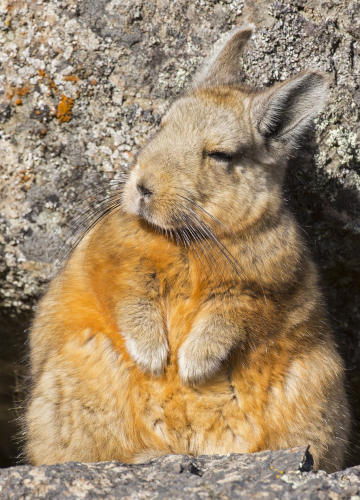
\includegraphics[scale=0.75]{../../../../../pictures/viscacha.png} \\
    \end{tabular}
\end{frame}

\subsection{Python}
\begin{frame}
    \frametitle{Python}
    \begin{itemize}
        \item universal high-order programming language
        \item good readability
        \item free
        \item runs on: \\
        \quad \\
        \begin{center}
            \begin{tabular}{ccc}
                
\includegraphics{../../../../../pictures/windows_logo.png} \hspace{1cm} &
                
\includegraphics{../../../../../pictures/macos_logo.png} \hspace{1cm} &
                
\includegraphics{../../../../../pictures/linux_logo.png}
            \end{tabular}
        \end{center}\\
        \quad \\
        
    \end{itemize}
\end{frame}


\begin{frame}
    \frametitle{Python - Anaconda (recommendation)}
    \begin{columns}
        \begin{column}{.5\textwidth}
            
\includegraphics[scale=0.5]{../../../../../pictures/anaconda_logo.png}
        \end{column}
        \begin{column}{.5\textwidth}
            \begin{itemize}
                \item \href{https://www.anaconda.com/products/distribution}{\textbf{Anaconda distribution}} for Windows, MacOS and Linux
                \item Python-centered, but supports also R
                \item easy handling of environments
                \item powerful package manager
                \item latest stable packages
            \end{itemize}
        \end{column}
    \end{columns}
    

\end{frame}


\subsection{ema2wav}
\begin{frame}
    \frametitle{ema2wav}
    \begin{itemize}
        \item converts EMA data into multichannel WAV-files (\& CSVs)
        \item Python-based, only free \& open-source dependencies
        \item supports AG500/501 (Carstens Medizinelektronik GmbH)
        \item multiple options for derivations \& calculations
        \item GUI, command line or python module
        \item work-in-progress
        \item .dmg (MacOS) \& script ($\leftarrow$ always latest version)
        \item can be obtained \href{https://github.com/phbuech/ema2wav}{\textbf{here}}
    \end{itemize}
\end{frame}

\end{document}


\begin{frame}
    \begin{center}
        \vspace{2cm}
        \begin{LARGE}
            1 - ema2wav \& Praat
        \end{LARGE}
    \end{center}
\end{frame}

\documentclass[12pt,a4paper]{beamer}
\usetheme{Montpellier}
\usepackage[utf8]{inputenc}
\usepackage[english]{babel}
\usepackage{amsmath}
\usepackage{amsfonts}
\usepackage{amssymb}
\usepackage{makeidx}
\usepackage{graphicx}
\usepackage{lmodern}
\usepackage{kpfonts}
\usepackage{fourier}
\usepackage[left=2cm,right=2cm,top=2cm,bottom=2cm]{geometry}

\begin{document}

\section{Program start}
\begin{frame}
    \frametitle{Program start}
    ema2wav can be started either
    \begin{itemize}
        \item using the \textbf{GUI}
        \begin{itemize}
            \item via binary (.dmg)
            \item via console
        \end{itemize}
        \item using command-line (see documentation)
        \item by importing as a python module (custom script/notebook/\textbf{Google colab notebook}; see documentation)
    \end{itemize}
    
\end{frame}

\section{User input}
\begin{frame}
    \frametitle{User input}
\end{frame}

\end{document}

\begin{frame}
    \begin{center}
        \vspace{2cm}
        \begin{LARGE}
            3 - Hacks
        \end{LARGE}
    \end{center}
\end{frame}

\documentclass[12pt,a4paper]{beamer}
\usetheme{Montpellier}
\usepackage[utf8]{inputenc}
\usepackage[english]{babel}
\usepackage{amsmath}
\usepackage{amsfonts}
\usepackage{amssymb}
\usepackage{makeidx}
\usepackage{graphicx}
\usepackage{lmodern}
\usepackage{kpfonts}
\usepackage{fourier}
\usepackage{hyperref}
\usepackage{tipa}
\usepackage[left=2cm,right=2cm,top=2cm,bottom=2cm]{geometry}
\beamertemplatenavigationsymbolsempty

\begin{document}

\section{Annotations}
\begin{frame}
    \frametitle{Annotations}
    \centering
    \begin{Large}
        Why use IPA for annotations?
    \end{Large}
\end{frame}

\subsection{character encoding schemes}
\begin{frame}
    \frametitle{Encoding}
    \begin{itemize}
        \item IPA symbols in Unicode (latin character, IPA extensions, Phonetic extensions)
        \item Whats the problem?
        \item different character encoding schemes:
        \begin{itemize}
            \item ASCII
            \item UTF-8
            \item UTF-16
            \item UTF-32
        \end{itemize}
    \end{itemize}
\end{frame}

\begin{frame}
    \centering
    \includegraphics[scale=0.4]{../../../../../pictures/ascii.png}
\end{frame}

\begin{frame}
    \centering
    \includegraphics[scale=0.2]{../../../../../pictures/utf16.png}
\end{frame}

\begin{frame}
    \centering
    \includegraphics[scale=0.5]{../../../../../pictures/compare.png}
\end{frame}

\begin{frame}
    \begin{center}
        {\LARGE \c{c}}
    \end{center}
    \begin{itemize}
        \item How many glyphs?
    \end{itemize}
\end{frame}

\begin{frame}
    \begin{center}
        {\LARGE \c{c}}
    \end{center}
    \begin{itemize}
        \item How many glyphs?
        \item U+00E7
        \item c (U+0063) + \c{\quad} (U+0328)
    \end{itemize}

\end{frame}

\begin{frame}
    \begin{itemize}
        \item ASCII and UTF-8 are compatible
        \item UTF-16 is not compatible with UTF-8
        \item but:
        \begin{itemize}
            \item UTF-8 with or without BOM
            \item UTF-16 Big Endian (Mac) vs UTF-16 Little Endian (Windows) (UNIX vs NUXI)
        \end{itemize}
        \item Why is this important?
        \begin{itemize}
            \item archiving of your data
            \item data sharing with collaborators
        \end{itemize}
    \end{itemize}
\end{frame}

\subsection{Praat}
\begin{frame}
    \frametitle{Text encoding in Praat (text writing)}
    \centering
    \includegraphics[scale=0.5]{../../../../../pictures/textwriting.png} 
\end{frame}

\begin{frame}
    \frametitle{Text encoding in Praat (text reading)}
    \centering
    \includegraphics[scale=0.5]{../../../../../pictures/textreading.png} 
\end{frame}

\subsection{Recommendations}
\begin{frame}
    \frametitle{Recommendations}
    \begin{itemize}
        \item uniform encoding
        \item X-Sampa
    \end{itemize}
\end{frame}

\begin{frame}
    \centering
    \includegraphics[scale=0.2]{../../../../../pictures/xsampa.png}
\end{frame}

\subsection{Hack for forced alignment}
\begin{frame}
    \centering
    {\LARGE Hack for forced alignment}
\end{frame}

\begin{frame}
    \centering
    \includegraphics[scale=0.3]{../../../../../pictures/audacity1.png}
\end{frame}

\begin{frame}
    \centering
    \includegraphics[scale=0.3]{../../../../../pictures/audacity2.png}
\end{frame}

\begin{frame}
    \centering
    \includegraphics[scale=0.3]{../../../../../pictures/audacity3.png}
\end{frame}

\begin{frame}
    \centering
    \includegraphics[scale=0.3]{../../../../../pictures/audacity4.png}
\end{frame}

\begin{frame}
    \centering
    \includegraphics[scale=0.3]{../../../../../pictures/audacity5.png}
\end{frame}

\begin{frame}
    \centering
    \includegraphics[scale=0.3]{../../../../../pictures/audacity6.png}
\end{frame}

\begin{frame}
    \centering
    \includegraphics[scale=0.3]{../../../../../pictures/audacity7.png}
\end{frame}

\begin{frame}
    \begin{itemize}
        \item use a script to extract the utterances of interest
        \item have one wav and one text file per utterance
        \item use the forced-alignment system of your choice
    \end{itemize}
\end{frame}

\end{document}


\end{document}